%%%%%%%%%%%%%%%%%%%%%%%%%%%%%%%%%%%%
% This is the template for submission to MICRO 2019
% The cls file is modified from 'sig-alternate.cls'
%%%%%%%%%%%%%%%%%%%%%%%%%%%%%%%%%%%%

\documentclass{sig-alternate}
\usepackage{mathptmx} % This is Times font

\usepackage{fancyhdr}
\usepackage[normalem]{ulem}
\usepackage[hyphens]{url}
\usepackage[sort,nocompress]{cite}
\usepackage[final]{microtype}
\usepackage{flushend}
% Always include hyperref last
\usepackage[bookmarks=true,breaklinks=true,letterpaper=true,colorlinks,linkcolor=black,citecolor=blue,urlcolor=black]{hyperref}




% Packages and commands not in template
\usepackage[dvipsnames]{xcolor} %color package
\usepackage{pifont} %check and x font
\newcommand{\cmark}{\textcolor{ForestGreen}{\ding{51}}}%
\newcommand{\xmark}{\textcolor{red}{\ding{55}}}%

\usepackage{float}



% Ensure letter paper
\pdfpagewidth=8.5in
\pdfpageheight=11in

%%%%%%%%%%%---SETME-----%%%%%%%%%%%%%
\newcommand{\microsubmissionnumber}{580}
%%%%%%%%%%%%%%%%%%%%%%%%%%%%%%%%%%%%

\fancypagestyle{firstpage}{
  \fancyhf{}
  \renewcommand{\headrulewidth}{0pt}
  \fancyhead[C]{\vspace{15pt}\normalsize{MICRO 2019 Submission
      \textbf{\#\microsubmissionnumber} -- Confidential Draft -- Do NOT Distribute!!}} 
  \fancyfoot[C]{\thepage}
}

\pagenumbering{arabic}

%%%%%%%%%%%---SETME-----%%%%%%%%%%%%%
%\title{Register File Cache: Efficient Memory Disambiguation and Pipeline Prefetching} 
\title{Efficient Temporal and Spatial Load to Load Forwarding} 
%%%%%%%%%%%%%%%%%%%%%%%%%%%%%%%%%%%%

\begin{document}
\maketitle
\thispagestyle{firstpage}
\pagestyle{plain}




\begin{abstract}
%{\color{red} Recent load value prediction techniques improve IPC by predicting load addresses and prefetching the data into the pipeline. This achieves the same zero load-to-use latency as an all-instruction value predictor but with simpler CPU components making more feasible to implement in hardware. However, it comes with a great increase in pressure in the physical register file and L1 cache in order to validate predictions. %Register reuse techniques could help mitigate the problem by providing load-to-load forwarding, but as we show in this work, state-of-the art register reuse techniques only take minimal advantage of the reuse potential.
%In this work, we make two observations: (1) the value predicted address are special and that the validation of most predicted addresses do not require the load to be replayed to validate the prediction, most of the CPU components required to validate the predicted load are already present in the CPU to detect memory ordering violations; and (2) due to having addresses early in the pipeline, we can easily cache, manage and detect data reuse, and perform load-to-load forwarding through the physical register, further decreasing register and cache pressure. %The address prediction components provided by load value predictors solves this issue by making load addresses available at decode and allows for a more effective register reuse detection and forwarding technique since it is based on load addresses, i.e. the same strategy used in any other cache level in the memory hierarchy.
%Our proposed address based register reuse technique improves data forwarding through the register file by 2.2x on average compared to a instruction-distance register sharing strategy. Moreover, it preserves the pipeline prefetching performance benefits while, not only nullifying the extra load instructions associated with it, but actually reducing the total number of load instructions executed by 36\%.}

During the execution of a program, many loads in close proximity in the dynamic instruction stream access the same or nearby addresses. While caching is the primary technique to exploit such temporal and spatial locality there is a limit on how close we can bring it to the pipeline. Ideally we would like to make the register file a ``cache'' but this is plagued by many problems.
We present a novel technique, which is a generalized form of load-to-load forwarding that captures both the spatial and temporal reuse of load instructions via the register file.

The key to an effective load-to-load forwarding technique is to prefetch L1 data into the register file early. For this we use load address prediction that is shown to offer good coverage for loads. Using predicted addresses, we prefetch a block of data, as it is readily available on the L1 bus, to capture spatial locality and pre-load registers with multiple values. We establish a connection between the addresses that are prefetched and the register tags via a helper structure that also manages the spatial and temporal reuse of the pre-loaded registers for future loads. Our temporal reuse is not limited to loads that coexist in the processor's instruction window but significantly exceeds this limit. Finally, we validate all prefetching, and load-to-load forwarding when we generate the actual addresses of the loads. We combine addresses, instruction sequence numbers (that represent program order), and store filtering to reduce the validation to mostly address comparisons and only rarely needing to re-access the cache to verify values.

The end result is that we are able to capture a significant part of the  reuse of loads that is available during the execution of a program (98\% of the locality available in the instruction window) while at the same time reducing the number of executed loads by 36\%. 

\end{abstract}




\section{Introduction}
%Single thread performance is still imperative in modern applications and CPU architectures need keep improving in this area. 
Satisfying loads as early as possible is of critical importance to performance. Not surprisingly, a plethora of micro-architectural techniques have been proposed towards this goal. Unfortunately, in many cases, achieving the desired effect with a technique also means undesired consequences, e.g.,: compromising energy efficiency or exerting increased pressure onto the memory system. 

In this paper, we re-revisit the interface of the core to the cache hierarchy (i.e., L1). We are not concerned on how to reduce the number of cache misses or the cost of each miss --- or more generally the mean time to access memory. Such techniques are orthogonal to our work. What we are concerned here is to optimize the latency starting from accessing data in L1 all the way to using such data in a load-dependent instruction. We aim to view the problem from a new perspective: 
%Satisfy as many loads as we can, as early as possible, by: i) making the best use of the mechanisms and datapaths that already exist in a typical out-of-order microarchitecture; ii) adding as little as possible in terms of helper structures, and iii) avoiding overtaxing other resources such as the ports to the L1.
generalized \emph{load-load forwarding}. Store-load forwarding is well known and researched, however load-load forwarding has been given less attention. We aim to generalize load-load forwarding both for temporal locality (spanning a chain of multiple loads) and spatial locality, i.e., feeding multiple loads with neighboring addresses from a block of data prefetched by a single load.

Historically, one approach for the problem of load latency has been to bring the cache hierarchy inside the core in the form of a faster L0~\cite{FilterCache/kin97, FilterCache2/bellas99, FilterCache3/giorgi07}. However, this does not fundamentally change the way we satisfy loads.  Loads still have to generate their effective address and access the L0 in the address name space. The benefit, however, is \emph{temporal and spatial reuse} (multiple loads can benefit from a cacheline containing multiple values in the L0) without any added complications in terms or instruction ordering or validation. 

A more radical approach that completely abandons the address name space, is to use value prediction (VP)~\cite{VP/lipasti96exceeding, VP/lipasti96value, VP/wang97highly, VP/tuck05multithreaded, VP/perais14eole, VP/perais15bebop}. VP tries to guess the result of an instruction, in the case of a load, VP predicts the value loaded. More broadly, VP allows instructions to proceed with predicted operands without waiting for the instructions that create these operands to execute. This \emph{speculatively} breaks true data dependencies and thus has the potential to increase instruction level parallelism (ILP) beyond the dataflow limit.
While promising, this technique comes with the caveat that mispredictions are costly so predicted values are only used when the prediction has a high confidence. This results in low coverage. Furthermore, since stores change the values in memory, they can interfere with predictions. This further decreases confidence in the prediction (and in coverage).
Load VP circumvents both the address name space and the register name space, predicting values and writing them directly into the destination register or forwarding them to waiting dependent instructions. However, as a prediction, VP needs to validate the predicted value by comparing it with the actual value accessed through the address name space. This means that a value-predicted load will execute and access the L1 and compare its loaded value to the predicted value. The benefits of temporal and spatial reuse are also not readily available in this case.
 
Sheikh et al.~\cite{DLVP/sheikh17} make the observation that addresses are easier to predict than data, and propose the \textit{Decoupled Load Value Prediction} (DLVP) technique that predicts the load addresses instead of the load values and prefetches the data into the pipeline just in time to be consumed by the dependent instruction(s). This effectively achieves the same zero load-to-use latency of a value-predicted load, but with increased coverage for load instructions, fewer number of iterations to trust the prediction, and fewer mispredictions due to stores changing the predicted value (mispredictions still occur when the store is out-of-order with respect to the access of the value but that is a more rare occurrence than the mispredictions of a value-prediction approach).
While effective this technique also significantly increases accesses to memory since every predicted load address needs to access the memory twice, once to prefetch and a second to validate the result in case of coherence or memory ordering violation. 
In contrast to value prediction, address prediction still maintains a connection to the address name-space, loading actual values from the predicted memory addresses.

In contrast to both VP and DLVP, \emph{register sharing} techniques~\cite{RS/jourdan98novel, RS/petric02three, RS/petric05reno, RS/fahs05continuous, RS/perais16register} work in the \emph{register name space}. In these techniques the address name space is used to establish a connection between instructions that effectively access the same address and instead of communicating via the cache hierarchy where the values are mapped on their respective memory addresses, they communicate via the register file where a value is \emph{mapped} after being loaded from its address into a register.
%The seminal example is the speculative memory cloaking and bypassing techniques by Moshovos and Sohi~\cite{MD/moshovos97}, where a connection is established (via the address name space) between a load that is memory-dependent on an earlier store. Communication between future instances of the store and the load is then \emph{speculatively} routed via the register file as soon as the store value is available (without the need to have the addresses). There is no need to access the actual value from the address name space (assuming the value can only change by stores of the same thread), but the addresses of the store and the load eventually must be compared to verify the speculation. 

%A limited form of load-load forwarding are \emph{register-sharing} techniques that allow forwarding between loads via shared registers. These techniques establish a connection in the register name space between loads that access the same address. 
These techniques are limited both in temporal locality (i.e. the locality exposed by the instruction window) and of course they cannot exploit any spatial locality as they deal with one value (mapped on a register) at a time.
A further complication, here, is to account for local and remote stores (that make their presence known via invalidations). Without continuously keeping track of the correspondence between the address space and the register space,  eventually requires \emph{value validation}: all loads must actually load their value from the memory system, in the correct order, and verify that the value they received speculatively via register sharing was correct.
%---validating by comparing addresses is not enough.

To summarize, the patterns that emerge from prior work are the following:
\begin{itemize}
\item Sticking to the address name space easily provides spatial and temporal reuse with no added complications ( there is no need for validation) but it prevents us from optimizing further as loads execute in their usual fashion: one by one and only after generating their address to access their value.
\item VP circumvents the address space but it has to be conservative to be accurate (mispredictions cost). In addition it has to be \emph{value-validated} via the address name space, so eventually it costs the same (or slightly more) with respect to accesses to the cache.
\item Register-sharing techniques, a from of limited load-load forwarding, also circumvent the address space and allow (limited) temporal reuse of values but spatial locality is not exploited. In addition, without keeping track of the correspondence of the register name space to the address name space, \emph{value-validation} of every individual load that shared a register with a previous load, is our only option.
\end{itemize}
%Moreover this technique misses one great advantage of having addresses early on in the CPU pipeline, which is the ability to take advantage of temporal and spatial data locality available in memory.
In this work, we aim to make use of the temporal and spatial reuse benefits of an address-based approach with the advantage of a \emph{generalized load-load forwarding}. To achieve this we need to solve two problems:
i) how to establish temporal and spatial reuse among loads as soon as possible so that only one access to memory to prefetch data is required; ii) how to validate this reuse. To provide an efficient solution to these problems we need an efficient way to establish a relation between the register space and the address space and an efficient way to validate the reuse without resorting to the replay of all loads to validate their value.
In broad terms, our approach is as follows:
\begin{itemize}
\item We predict load addresses and not values. Predicting addresses provides high accuracy with a much wider coverage~\cite{DLVP/sheikh17, AVPP/orosa18} very early in the pipeline.
\item We exploit temporal and spatial reuse by fetching from a predicted address multiple values (a cache sub-block) and mapping them on physical registers. Multiple subsequent loads can share these registers.
\item We keep the correspondence between the register name space and the address name space in a separate small structure, indexed by address, (called AT-RT) that also serves as the structure that keeps track of temporal and spatial reuse.
\item Lastly, we validate the loads only using their effective address once it is computed, \emph{without needing to access the cache for the value (no value-validation)}. 
Inspired by the \textit{Store Vulnerability Windows} (SVW)~\cite{SVW/roth05}, we use a simplified structure to detect possible memory dependence violations between loads and stores only having their address and program order. External invalidations from remote stores are handled by the load queue as in the baseline architecture.
\end{itemize}

%Based on the observation that predicting addresses enables us to do more than increase value prediction coverage. By using addresses we're able to validate most predictions without having to the re-execute the load instructions, since we can detect most memory violations using addresses alone, reducing register and L1 pressure; and we can detect data temporal reuse naturally and manage it in the register file, reducing register and L1 pressure even further and beyond state of the art register sharing techniques. Since applications also expose a great degree of spatial reuse, in some cases we're even able to expose more locality than the theoretical maximum available in the window provided by the load queue. 

Our solution is able to forward 36\% of the loads, compared to the 16\% of a state-of-art register-sharing technique, capturing 98\% of the load-to-load locality available in the pipeline. Compared to pipeline prefetching, that replays all the loads that prefetches, our solution not only manages to avoid replaying most prefetched loads, but also avoid executing the prefetch loads that have their data forward from the register file instead. This effectively reduces the total number of executed loads by 35\% compared to non-pipeline prefetching CPU. All this is done without sacrificing any of the performance benefits of doing pipeline prefetching.   


%\begin{figure}[ht]
%\centerline{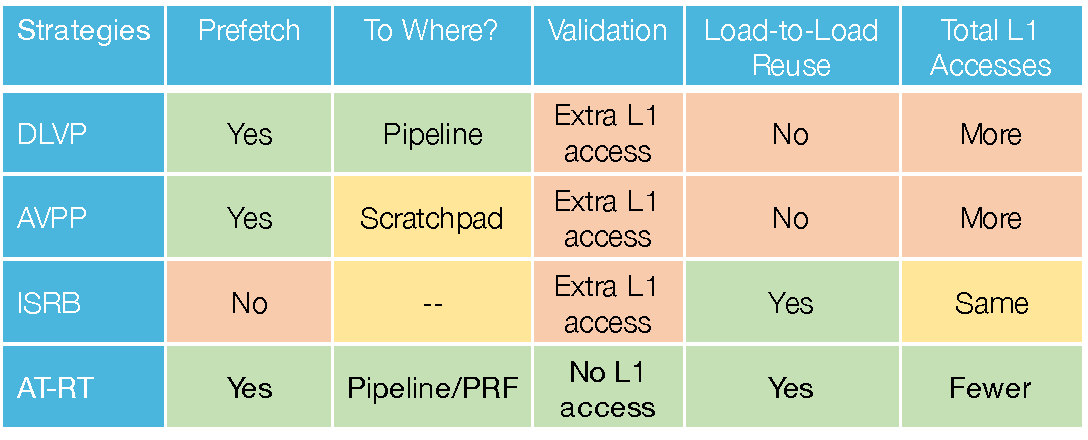
\includegraphics[width=0.50\textwidth]{diagrams/VsTable.pdf}}
%%\captionsetup{justification=centering}
%\caption{Table motivating our work}
%\label{fig:DistVsValue}
%\end{figure}





























\section{Background}

\subsection{Register sharing}
Register sharing was originally proposed by Jourdan et al.~\cite{RS/jourdan98novel} to eliminate register moves by doing register renaming. Their mechanism detects register reuse between instructions, renames said registers as the source registers of new instructions, and tracks the lifetime of the shared registers with reference counters. Several techniques have been proposed to improve the efficiency of register tracking and sharing~\cite{RS/roth2008physical, RS/battle2012flexible, RS/perais16register}. Perais et al.~\cite{ISRB/perais16} proposed the \textit{Inflight Shared Register Buffer} (ISRB) to improve reuse detection and simplify register tracking, but also enable load-to-load data forwarding through the register file. While such load-to-load forwarding is similar to our proposal, they require cache accesses to validate the values of data forwarded to loads . 

%While eliminating register moves is orthogonal to our approach, ISRB also allows for load-to-load reuse prediction and forwarding which overlaps with our proposal. Because of this, we compare our proposal to ISRB.

\subsection{Detecting memory ordering violations}
Memory ordering violations can come in two forms: \textit{internal}, where a load incorrectly bypasses an older store on which the load depends, and, \textit{external}, due to memory consistency model violations, typically appearing as coherence invalidation requests that catch speculatively performed loads out of their correct memory order.

Internal memory violations happen because processors allow loads to bypass independent stores for performance~\cite{MD/chrysos1998memory, MD/kessler1999alpha, MD/moshovos1997dynamic}. However, this bypassing happens before addresses are available, and is therefore speculative, based on a prediction of the load's dependence on older stores.  If the prediction is incorrect, the load and its dependency chain (or more commonly all following instructions) need to be replayed. External memory ordering violations can occur due speculatively reordered accesses that happen to conflict with external accesses. This is handled by tracking incoming coherence events. Even if no misprediction occurs within the core, the order of memory requests might still violate the consistency model due to other memory requests happening in parallel on other cores.

Ordering violations can be solved with a \emph{value-based approach}, which does a brute-force re-execution of every speculative load at commit to compare the loaded value with the speculative value. This comes with the cost of extra memory/cache accesses, which can have a significant impact on performance and energy. 
To address this problem strategies have been proposed to validate most memory bypassing and coherence events while minimizing the replaying of loads~\cite{RS/petric02three, MD/onder2001load, MD/sodani1997dynamic}. For detecting internal violations, we implement the \textit{Store Vulnerability Window} (SVW)~\cite{SVW/roth05} that avoids over 99\% of the replays in our results. 

To detect external memory violations, the load queue of the CPU holds the physical addresses of each load and is exposed to coherence traffic and invalidation requests, generating replays on hits. Virtual addresses are stored in both the load queue and the store queue to facilitate store-to-load forwarding and detection of internal memory ordering violations, since they are available sooner than physical addresses and using them can thereby reduce the penalty of mispredictions.     

\subsection{Value-prediction}
Value prediction techniques can be divided into two classes: \textit{computation-based} (such as stride predictors~\cite{SP/eickemeyer93load, SP/gabbay96speculative}) and \textit{context-based} (such as VTAGE~\cite{VP/perais2014VTAGE} and DVTAGE~\cite{VP/perais15bebop}). Orosa et al.~\cite{AVPP/orosa18} recently proposed an hybrid that merges a stride predictor with DVTAGE to improve on both.   

While value prediction is possible, it turns out that predicting the \textit{addresses} of loads is easier. First, addresses have simpler patterns, which increases prediction coverage. Second, since only about 25\% of instructions are loads, the predictor does not need to store nearly as much state~\cite{AVPP/orosa18}, making the prediction mechanism smaller and less complex. Recent work on load address predictors have shown they achieve the same performance benefit as prediction all values~\cite{DLVP/sheikh17, AVPP/orosa18}.
































%\section{Pipeline prefetch, register-sharing shortcomings}
\section{Motivation}
\label{sec:motivation}
%In this section we explain some of the factors behind our approach. 

Value prediction can avoid structural hazards by predicting results before they can be computed, allowing subsequent instructions to execute earlier. However, value prediction requires the predicted instruction to be executed for validation at some point before it commits. In the case of load instructions, this has typically meant executing the load, fetching the data from memory, and comparing the memory value with the predicted value. If the values are equal, the prediction is deemed correct, if not, the instruction and its dependency chain are replayed. 

Address predictors guess the address of the load and \emph{prefetch} the value instead of guessing the value itself. However, prediction validation remains the same and requires memory to be accessed. This means that an address predictor requires two memory accesses per load, one to prefetch the data and a second to validate the prediction, which negatively impacts pressure to the L1 ports and energy. Address prediction and value prefetch will be most successful when as many predictions as possible can be made. This advocates for techniques to increase prediction coverage. However, increased prediction coverage aggravates the problem of pressure to the L1 ports and eventually hurts performance. Figure ~\ref{fig:PrefetchedLoads} shows the percentage of loads predicted and executed twice, i.e. the percent increase in memory accesses compared to a traditional non-address predicting and non-pipeline prefetching.
As it is evident from this figure, the percentage of loads that can be predicted is high (60\% on average) and can reach 90\%. For this frequent prediction and prefetching it is imperative to find a way to validate the prediction without accessing the cache to reduce pressure and energy.


\begin{figure}[ht]
\centerline{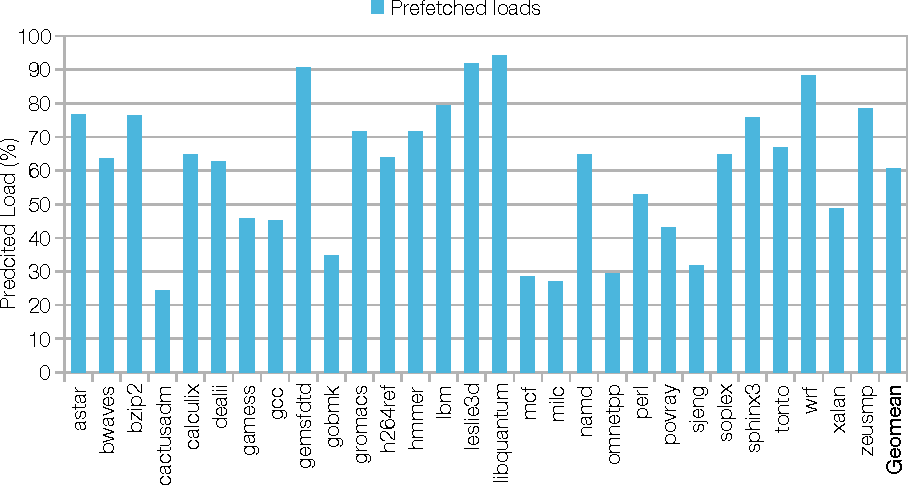
\includegraphics[width=0.50\textwidth]{graphs/PrefetchedLoads.pdf}}
\caption{Ratio of loads that a stride address load predictor covers and that DLVP would prefetch.}
\label{fig:PrefetchedLoads}
\end{figure}


\textit{Load-to-load forwarding} can mitigate this problem. One approach for forwarding is to store the results of the loads in a intermediate storage~\cite{nicolaescu2003, carazo2010l1, AVPP/orosa18} and validate the forwarding prediction from there. This is a similar strategy to having a filter-cache/L0 which requires extra data storage and data copies. Such strategies can perform well on applications with good locality, but have significant negative performance and energy impacts when there is not enough locality~\cite{SBAC-PAD/2017addressing}.  

Alternatively, one can take advantage of \textit{register sharing} techniques to perform load-to-load forwarding using the physical register file, which does not require extra data copies. Data is forwarded using the same physical register and only a single memory access needs to be made to validate the forwarded data. However, for this strategy to be successful, highly-effective reuse prediction is required. As figure~\ref{fig:IDistVsPotential} shows, tracking reuse by  \textit{instruction distance prediction}~\cite{ISRB/perais16}, can exploit less than half of the load-to-load forwarding potential that exists in the loads present in the load queue at any given time.

\begin{figure}[ht]
\centerline{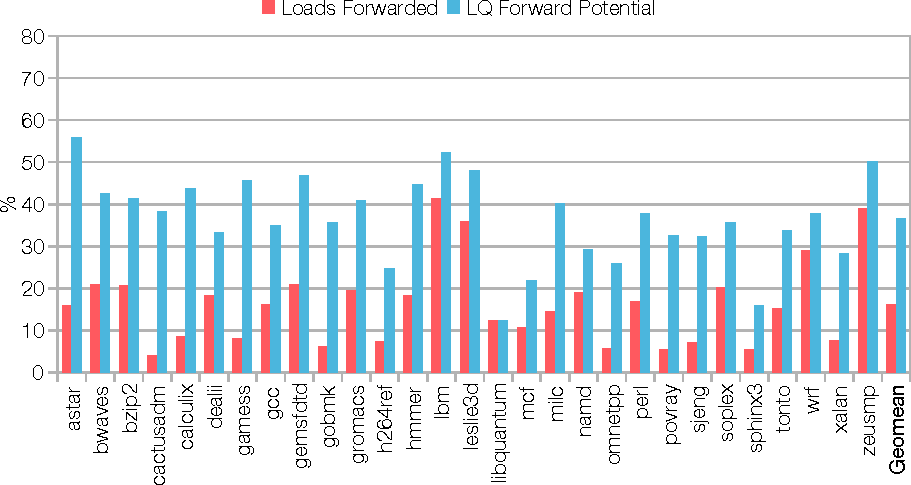
\includegraphics[width=0.50\textwidth]{graphs/IDistVsPotential.pdf}}
\caption{Ratio of loads that are forwarded using instruction distance to detect reuse, compared to total reuse potential available in the LQ.}
\label{fig:IDistVsPotential}
\end{figure}


While address prediction is an effective IPC improvement technique, it brings added pressure to the cache and register file since it requires accessing both structures on prefetch and validation. Register sharing can help mitigate the problem by sharing registers instead of prefetching and only accessing the cache for validation~\cite{ISRB/perais16}. However, proposed approaches that use instruction-distance have limited ability to take advantage of the reuse present in the register file and address prediction schemes suffer from significant increases in L1 pressure by having to validate based on values. %Even if coverage is perfect, it would only be able to match a non value-predicting pipeline memory accesses since all loads need to access the memory for validation.  

Our proposal leverages the fact the predicted loads have their address available as early as in the fetch stage (from the address predictor), and as such, it is possible to have the physical register file behave like a cache for this subset of load instructions. That is, we propose to detect data load-to-load reuse based on predicted addresses to avoid extra access to L1 and replication of data in the register file, and validate forwarding by comparing the predicted address to the generated one, thereby reducing L1 accesses and increasing reuse. Table~\ref{table:formatting} summarises the main characteristics of the different competing state-of-the-art techniques that will be discussed throughout this paper, and compares them with our proposal (bottom row).

\begin{scriptsize}
%\begin{table}[h!]
\begin{table*}[h!]
  \centering
  \begin{tabular}{|c|c|p{23mm}|p{23mm}|p{23mm}|p{23mm}|p{23mm}|p{23mm}|}
    \hline
    \textbf{Strategies} & 
    \textbf{Prefetch} & 
    \textbf{Granularity} & 
    \textbf{To Where?} &
    \textbf{Load-Load reuse} & 
    \textbf{Validation} & 
    \textbf{L1 accesses} \\ 
    %\textbf{comment}\\
    \hline
    
    \hline
    DLVP~\cite{DLVP/sheikh17} &  \cmark & {\color{orange}accessed \newline item (e.g., word)} & pipeline & \xmark &  {\color{red} Value-based} &  {\color{red} more}     \\
    \hline
    AVPP~\cite{AVPP/orosa18} &  \cmark & {\color{ForestGreen}next line} \newline (e.g., next word) & {\color{red}scratchpad} \newline (extra storage in LQ)  & \xmark & {\color{red} Value-based} &  {\color{red} more}    \\
    \hline
    % ISRB~\cite{ISRB/perais16} &  \xmark & -- & -- & \cmark ({\color{orange}single address} / {\color{ForestGreen}multiple loads}) & {\color{red} Value-based} &  {\color{black} same}     \\
    ISRB~\cite{ISRB/perais16} &  \xmark & -- & -- & \cmark ({\color{red}---} / {\color{ForestGreen}temporal}) & {\color{red} Value-based} &  {\color{black} same}     \\
    \hline
    % AT-RT &  \cmark & {\color{ForestGreen}block} \newline (e.g., 128 bits)& pipeline/PRF & \cmark ({\color{ForestGreen}multiple addresses} / {\color{ForestGreen}multiple loads}) &  {\color{ForestGreen} Address-based} & {\color{ForestGreen} fewer}     \\\hline
    AT-RT &  \cmark & {\color{ForestGreen}block} \newline (e.g., 128 bits)& PRF & \cmark ({\color{ForestGreen}spatial} / {\color{ForestGreen}temporal}) &  {\color{ForestGreen} Address-based / Value-based} & {\color{ForestGreen} fewer}     \\
    
    \hline

    
    \hline
  \end{tabular}
  \caption{Comparison of the different overlapping techniques considered in this work.}
  \label{table:formatting}
\end{table*}
\end{scriptsize}


%validates all predictions without requiring the second access to memory, effectively removing all validation memory accesses from the address value predictor. And by combining the new validation technique with register file sharing we are also able to remove some of the prefetch requests by forwarding the data from the register file, reducing the total memory accesses even than a standard on address predicting pipeline. Since we use the predicted addresses to detect reuse and forwarding potential, our solution also significantly increases the reuse potential available in the pipeline, reducing pressure in the register file and cache even further. 

























%\section{EFFICIENT PIPELINE PREFETCHING USING THE PRF AS A CACHE}
\section{Efficient, temporal load to load forwarding and prefetching}

The ability to accurately predict the address of a load just by seeing its PC in the fetch stage allows us to prefetch its value from the L1 directly into the register file. 
%We call this prefetching into the register file. 
We predict \emph{physical} addresses directly so we can prefetch without having to go through address translation first. Keeping the prediction in the physical address space helps with exposing the predictions to external conflicting accesses as we discuss later on. 

Prefetching into the register file works when the prefetch access is timed to deliver the value earlier or just in time when the dependent instruction(s) are ready to consume it, thus achieving a performance benefit from the shorter (or zero in the best case) latency. 
In addition, a place is needed to store the prefetched value to be able to filter further access to L1 (in this case, avoid executing any loads at all). While there are many alternatives for storage (e.g., an L0, the load queue, etc.) the physical register file is the most efficient choice, as it is the final destination for the data, and will avoid the overhead of intermediate copies. 

To effectively use the PRF as a cache we need to address two issues: we need to be able to 1) \emph{find} the prefetched data and 2) \emph{forward} them efficiently and without having to re-access the cache. 
This is achieved via a structure (explained in the following section) that establishes a connection between the address name space and the register name space and tracks the reuse of prefetched data by load instructions. 

Existing register reuse techniques suffer from limited coverage of the total potential for load-to-load reuse (as we showed in Section~\ref{sec:motivation}) and require accessing the cache to validate correctness. However, if we can make the PRF work as a cache, we can both improve the coverage and avoid the need to re-access the L1 for correctness. 

%To efficiently prefetch into the pipeline using the physical register file, one should aim to turn the PRF into a cache as much as possible. This means we should be able to forward data from the register file if the data is present (no extra data movement within the PRF), and be able to correctly and safely provide the data without accessing extra cache levels. Existing register reusing techniques can be used in an effort to achieve this, but only avoid the problem of the extra data movement (since they still require accessing the L1 for correctness), and even so, they have limited coverage of the total load-to-load reuse potential available.


\subsection{Finding and forwarding prefetched data via the Address Tag-Register Tag table}
To detect register reuse and perform load-to-load forwarding through the register file, we propose the introduction of a speculative register translation table (the \textit{Address Tag, Register Tag} (AT-RT) table) to assist load-to-load reuse \textit{based on addresses}, and associate those addresses to the register tags of the PRF that holds the data. This table is in essence a set of address tags and register tags for the data in the PRF that was pre-loaded from memory. The AT-RT is direct-mapped using the address as index. Each of its entries holds a register tag, a reference counter for the number of instructions that are sharing it, a valid bit, and an address tag. The table is indexed using the predicted address for each load, since this is provided by the load value predictor in the fetch stage.

The AT-RT is filled by load instructions that put their destination register tag and (predicted) address tag in the appropriate entry, increment the reference counter, and mark the entry as valid. When a later load instruction finds its predicted address in the AT-RT, it can skip allocating its own destination register and instead reuse the same register tag as the one found in the AT-RT by incrementing its reference counter. This allows subsequent loads to treat the PRF as a cache by detecting and reusing registers based on the address they correspond to.
Note that for all the above to happen it is essential that the predicted load address is available very early in the pipeline (e.g., in the fetch or decode stage, before register renaming begins).
%On a first access, since no entry is invalid, the load instructions go thought the normal renaming path, allocating a destination register. After a register is allocated, they record that register ID in the corresponding entry, increment the reference counter, update the tag, and mark the line as valid. When a following load instruction matches on a valid entry with its predicted address, the load instruction can skip allocating a new destination register and will just increment the entry reference counter and reuse the same register. 
When a predicted load commits, its reference counter in the AT-RT is decremented. When the reference counter reaches zero, i.e, no uncommitted loads are referencing that register tag, the entry is marked invalid.  We note here, that other techniques, such as move elimination (which is common in Intel CPUs), use reference counters in the physical register file. Reference counters in the AT-RT table are independent from the reference counters in the PRF. Thus, freeing an entry in the AT-RT does not automatically free the corresponding physical register. However, as we will show in subsequent sections, an AT-RT entry itself may behave as active user of a register (i.e., increment the register's reference counter) to prevent its de-allocation. 

%Even if a load deallocates an entry, it still also needs to decrement its own register(s) reference counters, these in turn will be deallocated if they are not being used by other (non-loads) dependent instructions. 

Predicted loads are inserted in the load queue with their respective predicted address. This tracking of the predicted address with the load enables efficient memory ordering violation detection based on the address, thereby eliminating the need to compare the value itself via an extra memory access. %The predicted address is fetched from the LQ for validation, just like a non-predicted load instruction (more details ahead).

%Each entry also holds the sequence number of the last loads that indexed it to deal with memory ordering issues (further discussion ahead).

\subsection{Forwarding validation}
Our approach relies on two types of predictions: (1) the load address, and (2) whether the load-to-load forwarding violates memory ordering, i.e, if there are conflicting stores between the loads. The first prediction can be easily validated when the load's address is finally generated. Validation compares the actual address to the predicted address, which only requires an access to the load queue (where the predicted address is stored). 

Recall that we predict in the physical address space so the computed address of the load needs to be translated before we access the load queue for the comparison. In any case, an access to the TLB is required to avoid synonyms and verify page permissions. As modern machines have first-level TLBs whose energy is an order of magnitude smaller than the L1, and this TLB request is required in the baseline design, we are not adding extra overhead.

Validating memory order is more involved and needs to be separated into external and internal violations. External ones come in the form of memory coherence invalidation requests. Although complex to solve, this type of ordering violations is present in all multi-core systems, and as such, the CPU already has mechanisms to detect the violating loads~\cite{SVW/roth05}, rollback the values of the shared registers~\cite{ISRB/perais16} and replay the infringing instruction chains~\cite{Bank/perais15}. The only extra step introduced by our approach is that the AT-RT also needs to be accessed to invalidate the entry for that address. Since the table is direct-mapped and indexed by physical addresses, this is a fast access to invalidate the entry. Is also relevant to mention that this negative coherence interaction can be completely avoided by delaying coherence requests in L1 without any loss of performance~\cite{ros2018superfluous}.

\begin{figure}[ht]
\centerline{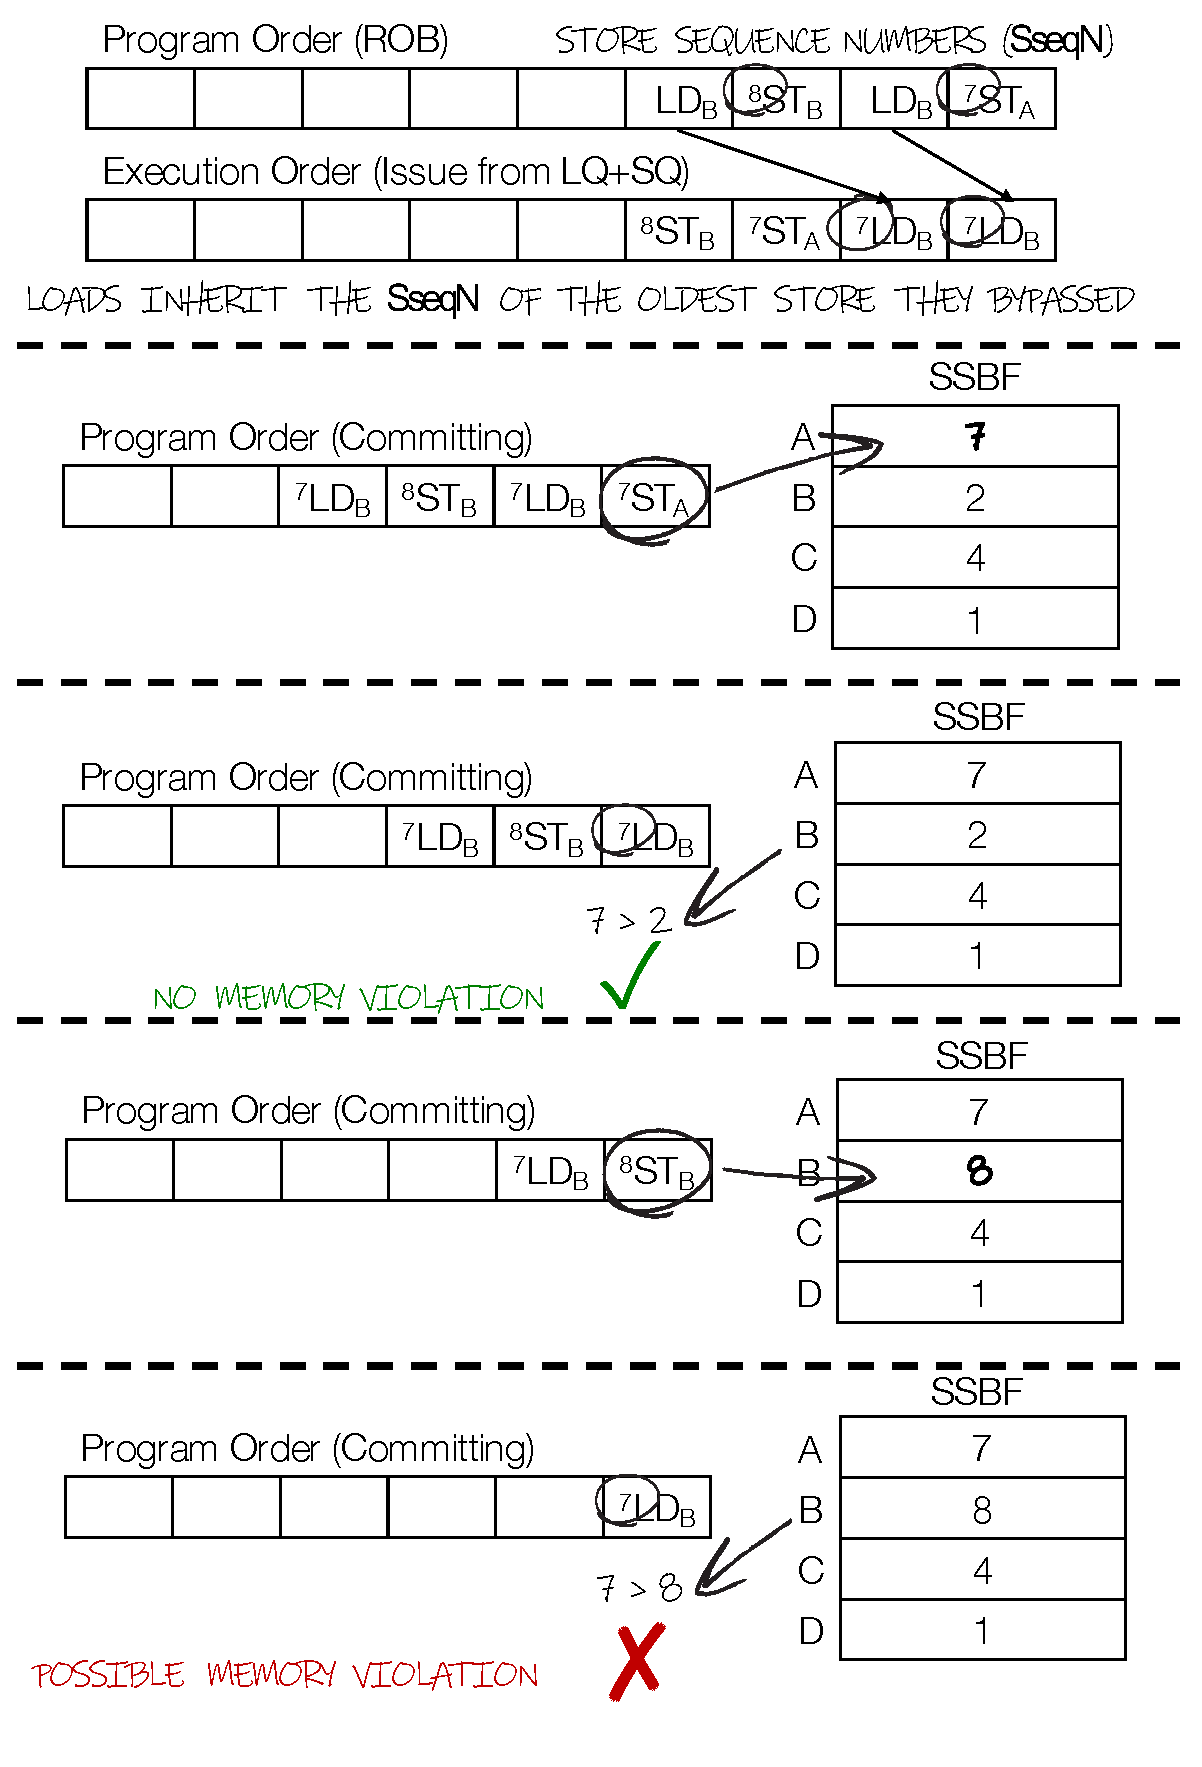
\includegraphics[width=0.50\textwidth]{diagrams/MemOrdValidation.pdf}}
\caption{Example of how the Store Sequence Bloom Filter (SSBF)~\cite{SVW/roth05} is used to detect possible memory ordering violations using Load/Store addresses (letters) and store-sequence-numbers (numbers)}
\label{fig:MemOrdValidation}
\end{figure}

In order to deal with internal memory ordering problems, we need to detect memory ordering violations. Our approach is independent of the memory dependency predictor. For this work we implemented the one proposed by A. Roth~\cite{SVW/roth05}, as it minimises redundant accesses accesses to the L1 to validate memory ordering by filtering loads that are not in a \textit{Store Vulnerability Window} (SVW). This mechanism relies on \textit{store sequence numbers} (SseqN) to detect if a load is in the vulnerability window of a store and only loads that are in the vulnerability windows need to be replayed. 

Figure~\ref{fig:MemOrdValidation} shows an example of how order is validated. At commit, and in program order, the stores update the SSFF table and loads check the SseqN of the youngest store that wrote to the same address. If the youngest store to write to that address is older than the store the load bypassed, than the issue order is valid, otherwise, there might have been a order violation and the load needs to be replayed. 
The example shows an execution order that has the first load correctly bypass an older store, and a second load correctly bypass one store (\(ST_A\)) but incorrectly bypass another store (\(ST_B\)). At commit, the infracting load is correctly detected since it bypassed an older store than the last one that wrote to same memory location.
 
%In the example in figure~\ref{fig:MemOrdValidation}, the second violating load only checks address B (despite bypassing a store to address A as well) and will always   
Load-to-load forwarding does not affect the scheduling and execution order of the associated loads, but by forwarding the data from older loads to younger ones, there is an implicit memory bypassing by the younger load. From a memory ordering point of view, both loads ``executed" at the same time. This can be an issue if there is a conflicting store between two loads with forwarding. To circumvent this problem, the SVW strategy needs to be modified, by having loads inherit the SseqN of the loads they had the data forwarded from, and thus inheriting their vulnerability window as well. 
This SVW modification is required by any load-to-load forwarding technique, not just the register file based one proposed in this paper. 


%This modified SVW strategy solves the problem of validating forwarded loads, but creates an issue with speculative memory bypassing since forwarded loads are bypassing intermediate memory instructions. This requires the forwarding mechanism to be aware of the memory ordering violations to avoid replays.   



\subsection{Interaction with the memory bypass predictor}
Any speculative forwarding technique needs to be informed by the speculative memory bypassing (SMB) predictor. Because, even if there are no correctness concerns, as incorrect schedules can be squashed, misspeculations and associated misschedulings can still have a profound impact in performance, requiring the pipeline to be flushed and instruction dependency chains to be replayed~\cite{alves2018dynamically, Bank/perais15}. 

%Load-to-load forwarding does not affect the scheduling of the associated loads, but by forwarding the data from older loads to younger ones, there is an implicit memory bypassing by the younger load. From a memory ordering point of view, both loads ``executed" at the same time. This can be an issue if there is a conflicting store between two loads with forwarding. 

For our solution we use the same \textit{Load Store Conflict Detector} (LSCD)~\cite{DLVP/sheikh17} strategy as DLVP to enable or disable forwarding for particular loads before rename. If the LSCD detects a forwarding conflict, it invalidates the corresponding entry in the AT-RT table, preventing following loads from having likely stale data forwarded.
Figure~\ref{fig:LSCD} shows an example of a typical memory ordering violation introduced by load-to-load forwarding and the correct forwarding combination. 


\begin{figure}[ht]
\centerline{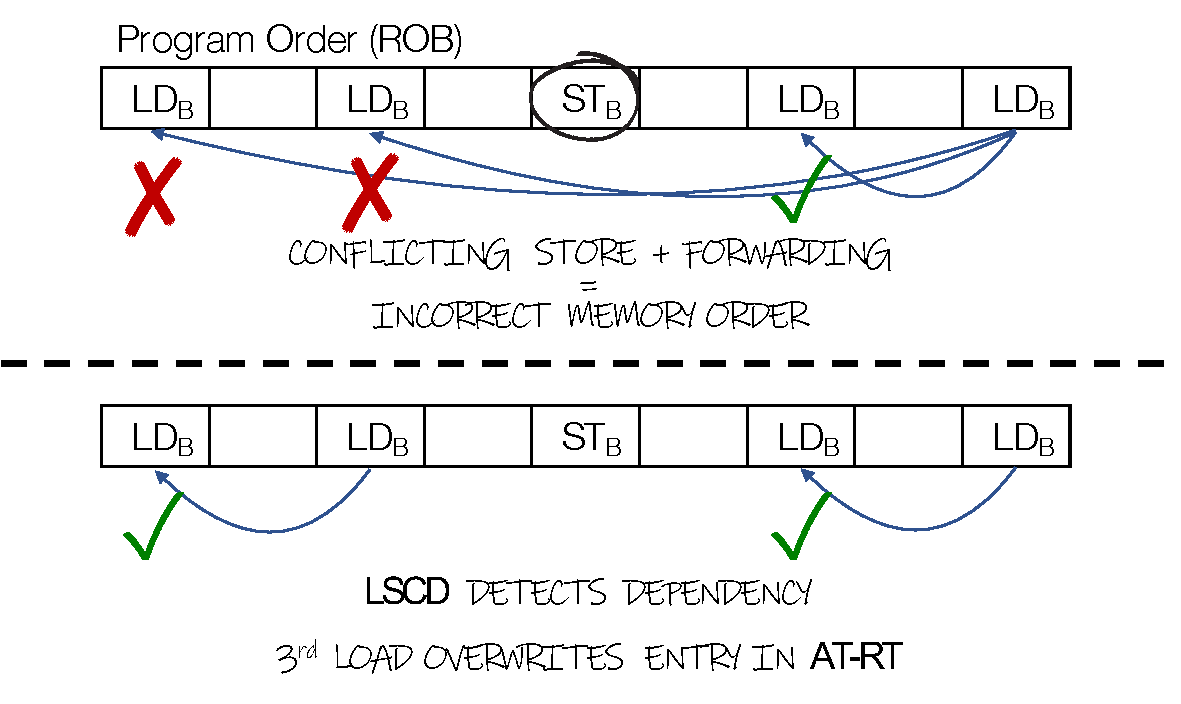
\includegraphics[width=0.50\textwidth]{diagrams/LSCD.pdf}}
\caption{Example of how forwarding can create a memory ordering violation even if execution follows program order. LSCD~\cite{DLVP/sheikh17} learns the memory violation and breaks the erroneous load-load forwarding to the 3rd and 4th loads by forcing the 3rd load to make a new entry in the AT-RT. This also enables the correct forwarding to the 4th load.}
\label{fig:LSCD}
\end{figure}


Perais at al.~\cite{ISRB/perais16} go one step further and break memory dependencies by identifying the producer of a load and renaming the destination register of the load as the source register of the producing store. This effectively allows for load-to-store forwarding through the register file as well as load-to-load. In this work we consider only load-to-load forwarding. Store-to-load forwarding from uncommitted stores is independent.


\subsection{Address prediction}
Our solution is independent of the chosen address predictor but needs the prediction early in the pipeline to manage register sharing and provide load-to-load forwarding through the PRF. For simplicity we chosen a stride based predictor. The prediction table is indexed by PC and each entry holds the last accessed address, the stride, and the confidence level (2-bit saturated counter). The prediction is only trusted when the counter is saturated. Details are described in section~\ref{sec:simulation}. 

Although highly accurate~\cite{AVPP/orosa18}, a stride predictor is not the most accurate predictor. (The most accurate in the literature is a hybrid DVTAGE~+~Stride value predictor~\cite{AVPP/orosa18}). However we found the stride predictor was accurate enough and provides a good baseline. It is important to note that more  sophisticated value predictors would increase coverage and/or decrease errors, improving our proposed solution even further.  





















%Coarse grain tags, to track 128-bit/sub-array-width chunks
\section{Exposing Spatial Locality via the PRF}
A key function of caches (indeed the main benefit of L0s) is that they expose spatial locality. While this is desirable for any cache hierarchy level, it seems unnecessary to do the same in the PRF when used in conjunction with prefetching, performance-wise. % and register sharing. 
Take for example DLVP: The performance benefit of having the spatial adjacent data already in the "cache level" before they are needed, is nullified by the prefetching of DLVP. Moreover, DLVP minimises cache pollution, since it will only fetch the data that it predicts it will be used instead of fetching and installing adjacent data (cache line granularity) on every access regardless of reuse.

While the performance benefit of spatial locality is likely to be covered by prefetching, the real benefit is to reduce energy. Unlike L2s and L3s that exchange data at fixed "cache-line" size blocks, L1s are optimised for small and variable data size granularity. Modern vector-load enabled CPUs can have busses to L1 as wide as 512-bits, to be able to satisfy large vector load instruction in a single access. %While the performance benefit of supporting such loads is clear, it is not obvious whether a wide cache load is more or less energy efficient than multiple small ones. 


\subsection{SRAM Cache Layout}

SRAMs are built as matrices of smaller sub-arrays and connected with h-tree shaped busses. Each sub-array is a group of SRAM cells, and the width of the sub-arrays determines the minimum number of bits read per cache access. These sub-arrays can be resized, but smaller sub-arrays (which have smaller minimum read-out widths) require larger numbers of sub-arrays to achieve the same capacity, and thus more complex h-tree. The smaller the individual sub-arrays and h-tree, the faster and more energy efficient an individual cache access can be. But since decreasing the sub-array size means increasing the h-tree complexity, the final design is usually a compromise (Figure~\ref{fig:sub-arrray}). For a first-level, 32KB, 8-way set associative cache, a 128-bit sub-array is a typical choice~\cite{SBAC-PAD/2017addressing, cacti-p11}, and we assume such a layout for this work.


\begin{figure}[ht]
\centerline{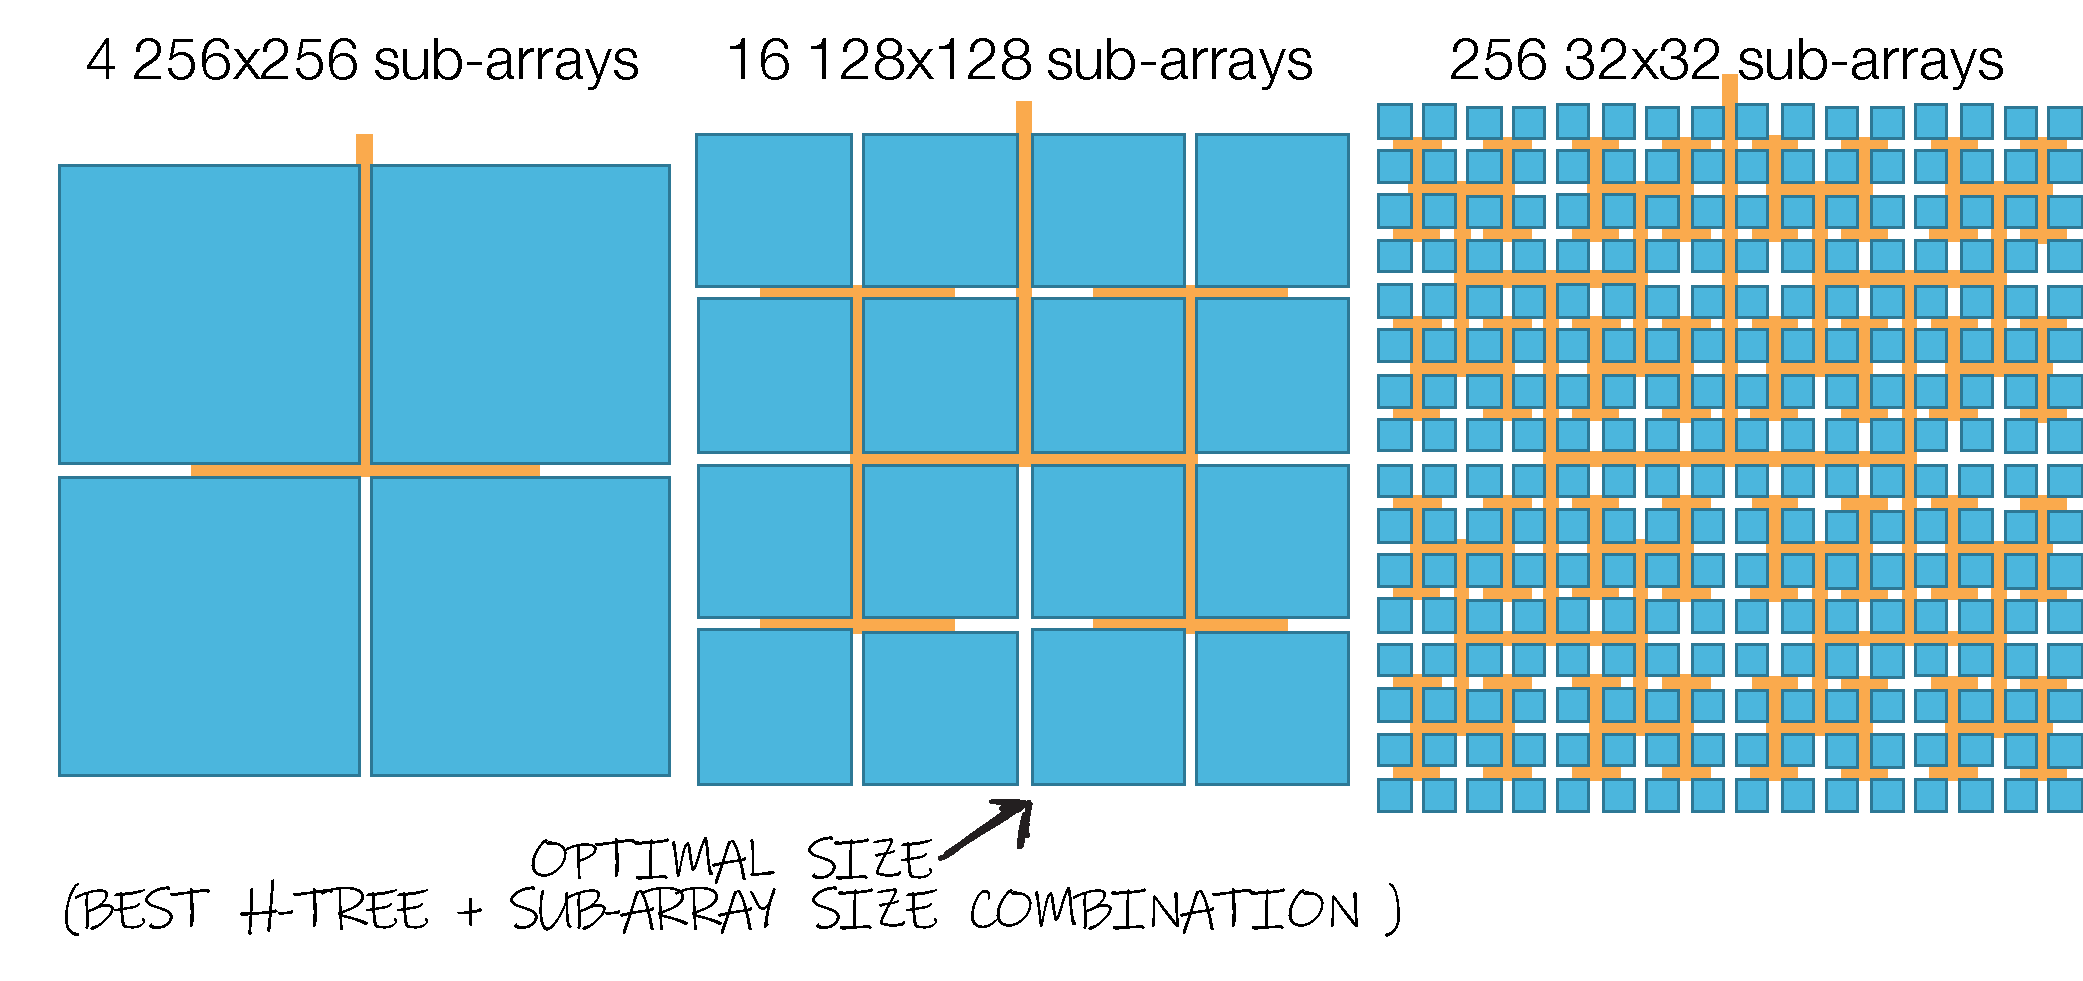
\includegraphics[width=0.50\textwidth]{diagrams/sub-array.pdf}}
\caption{32KB cache with using different sub-array size and respective h-tree combinations~\cite{SBAC-PAD/2017addressing}. The smaller the sub-array the smaller the minimum data read-out width, but the larger the overhead of the h-tree.}
\label{fig:sub-arrray}
\end{figure}


As the sub-array determines the SRAM read-out width independent of the load, all read-outs are 128-bits. This means that energy benefit of coalescing multiple loads into 128-bits can be substantial. For example, grouping two 64-bit requests into a single 128-bit one (if they access the same sub-array line) could avoid a second 128-bit read, and thereby half the cache access energy. In essence, this read-out constraint sets our optimal cache-access size when fetching data from L1.


\subsection{Coalescing loads efficiently}
While coalescing loads into 128-bit blocks seem appealing to minimise accesses to L1, there are two problems associated with it: (1) installing extra data that will not be used (extra writes and pressure in the PRF), and, (2) how to find the prefetched data in the PRF to provide it to later loads. Both of these problems can be solved by leveraging the predicted load addresses. (1) Since loads addresses are available speculatively in the front-end of the CPU, one can use those address to detect coalescing opportunities and only install the exact data from the 128-bit sub-array read-out into the PRF. Given the small prefetch range (128 bits), the time between rename and load write-back is enough to find most loads (also address predicted) that map to the same 128-bit block. (2) Since we only prefetch data for loads at or beyond the rename stage all loads will already have a destination register in the AT-RT table. As a result, the 128-bit sub-array read-out that returns from the cache can be stored in the different registers mapped by the AT-RT that match the sub-addresses of this block. The bytes of the 128-bit block that do not have a valid entry in the AT-RT by the time the load returns, are discarded.

To optimise for this type of access, the AT-RT table can be modified so that each entry now tracks the group of registers that contain any of the 128-bit block. Each then tracks multiple registers depending on the load size, e.g., 8, 4, 2 or 1 registers for load sizes of 1, 4, 8 or 16 (or more) bytes respectively. This mapping (although not required) matches how tracking is done in a typical cache (i.e. in blocks). This is also does not change the behaviour of tracking individual registers, since reference counting is done independently of how many registers each individual AT-RT table entry tracks. 




\subsection{Exposing more locality than the LQ provides}
Register lifetime is tracked by its reference counter in the PRF; it is incremented when a new instruction references it and decremented when it commits. Once the count reaches zero, the register is deemed free as far as the renaming logic is concerned. The reference counter in the AT-RT table follows the same strategy. The implication of this mechanism is that the forwarding potential of load-to-load forwarding is limited by the number of loads that can be tracked by the CPU at a given time. E.g., the larger the window of load instructions, the more forwarding is possible. The reuse potential for loads is therefore capped by the reuse windows exposed by the load queue, the CPU structure that tracks all the load instructions currently available in the CPU. The forwarding potential is also limited in previous register reuse techniques that are based on instruction distance by the largest distance that can be observed in the processor's instruction window.

%Existing register reuse techniques are based on identifying pairs of instructions that reuse the same data, for load-to-load reuse, this means that the pair needs to be present in the load-queue simultaneously to be identifies. for example, ISRB uses instruction distance to track reuse, if the distance is higher than the load-queue size, load-to-load forwarding is not possible. 

However, since we use addresses to detect reuse, the lifetime of the load instruction (and its registers) are no longer such a limitation. Even if a load retires and leaves the load-queue, it can still leave a valid entry in the AT-RT table. This means that another load, outside of the window of the load-queue can later be fetched, predicted to have the same address, and reuse the data in that register. However, this also means that a register can be ``freed" (reference count of zero) between reuses, thereby losing the potential reuse. 

%or (2) we do not let the retiring load decrement the reference counter and free the register for later (potential) use which causes an artificial pressure on the register file (how to decide which registers to hold and for how long?).

To address this problem we make each entry in the AT-RT table increment the PRF reference counter as well. This way, even if all instruction referencing the register (loads or otherwise) commit, the PRF will not free the register if there is still a valid entry in the AT-RT that can allow later loads to reuse its data. Invalidating the entry (either due to avoid memory ordering violations or a collision) requires the respective register reference counter to be decremented as well.

With this strategy alone, AT-RT lines can only be invalidated if another line maps to it (collision) or if a load-store collision is detected (LSCD unit). To allow the front-end of the CPU to free registers in case of increased register pressure we need to implement some sort of register garbage collection system. This system can be as simple as randomly invalidating lines when needed to a LRU replacement policy. Since we opted to track multiple registers per AT-RT entry for sub-array read-out coalescing, each entry has its own line reference counter for how many loads in the pipeline are referencing the current line (not individual registers of the line). As a result, the line is kept alive as long as there is at least one register of that line currently being referenced by an uncommitted load. This strategy does not maximise reuse, since we still might be freeing registers too soon and not seeing the full reuse potential available. However, it strikes a compromise between extending a register's lifetime and implementing a trivial mechanism to recover registers unreferenced registers. Since the AT-RT finds significant register reuse opportunities, even increasing the lifetimes of registers in the PRF in this manner does not increase overall register pressure. Infact, we did not  encounter a single situation where our approach used more registers than the baseline configuration.   


%This problem can be circumvented by levering adding an extra bit to reference counter in the register file, that indicates if a free register still has a valid entry in the register renaming table (the still valid bit). An invariant is that this bit is never set if the reference counter is bigger than zero.
























\section{Evaluation}
\label{sec:Results}

\subsection{Simulation and Modeling}
\label{sec:simulation}
We use 10 uniformly-distributed checkpoints for each SPEC2006~\cite{speccpu06} application. Checkpoints are warmed for 100M instructions and results extracted from 10M instructions of detailed simulation. We use gem5~\cite{gem5} to simulate a large out-of-order X86\_64 CPU (Intel Skylake-like 8-wide, 224 entry ROB, 72 entry LQ, full details in Table~\ref{table:cpu-specs}). The first-level cache is dual-ported with pipelined loads and stores. %For energy evaluations we use CACTI~\cite{cacti09} with a 22nm technology node~\footnote{For energy modeling, we model a 64 entry, 4-way set-associative dTLB to match the first-level TLB of the Intel Skylake architecture.}.

\begin{table}
	\begin{center}
	\begin{tabular} {|c|p{47mm}|}
    \hline
    Frequency & 3.6GHz \\
    %\hline
    IssueWidth/Ld,St Units  & 8/2,2 \\
    SQ/LQ/IQ/ROB & 56/72/50/224\\
    iTLB/dTLB & 512/512 fully-assoc\\
    \hline
    Value Predictor & Tagged 1K entry stride-predictor \newline table w/ 2-bit conf\\
    Memory Order Valid & Tagged 1K entry SSBF\\
    DDT (only for IDist) & Tagged 1K entry table\\
    \hline
    AT-RT & 512 entry table \newline
    Tag (48-bits), RegID (8-bits), \newline 
    ref-counter (5-bits), valid (1-bit)\newline 
    \textbf{Total size} 3968 Bytes\\
    \hline

    Caches & L1I/L1D/L2/L3 \\
    Size & 32KB/32KB/256KB/8MB \\
    Latency & 1c/2c/12c/38c \\
    Associativity & 8w/8w/8w/16w \\
    \hline
    DRAM & DDR3, 1600MHz, 64bits \\
    \hline
	\end{tabular}
    \end{center}
 % \captionsetup{justification=centering}
  \caption{Gem5 simulator configuration.}
  \label{table:cpu-specs}
\end{table}


We evaluate five configurations: 

\begin{itemize}
% \squishlist
\item \textbf{DLVP:} Address load predictor that prefetches the predicted loads.
\item \textbf{IDist:} Register reuse technique that uses instruction distance for load-to-load reuse (ISRB)\footnote{While the standard ISRB does not filter any load instruction, for a fair comparison, we include the SSBF filter in the IDist configuration as well.}. 
\item \textbf{AT-RT (Temp):} DLVP + Our register reuse technique that uses predicted addresses to forward data (temporal reuse).
\item \textbf{AT-RT (Temp+Spat):} DLVP + Our register reuse technique but with coalescing of loads to the same 128-bit sub-array read-out (temporal and spatial reuse).
\item \textbf{Baseline:} Pipeline with no pipeline-prefetching and no register reuse.
% \squishend
\end{itemize}


\subsection{Prediction accuracy}
The forwarding potential of AT-RT is a function of the available locality and the accuracy of the predictor. Figure~\ref{fig:VPAccuracy} shows the accuracy of our stride address predictor. The stride predictor shows high coverage, with the majority of the benchmarks (17) being able to accurately predict more than 60\% of the addresses, and 8 benchmarks having an accuracy above 75\%. Only 6 benchmarks have an accuracy bellow 40\% with \textit{cactusadm}, with only 24\% accuracy, being the benchmark with the lowest success ratio. On average, the predictor is able to accurately predict the address of 59\% of the loads.


\begin{figure}[ht]
\centerline{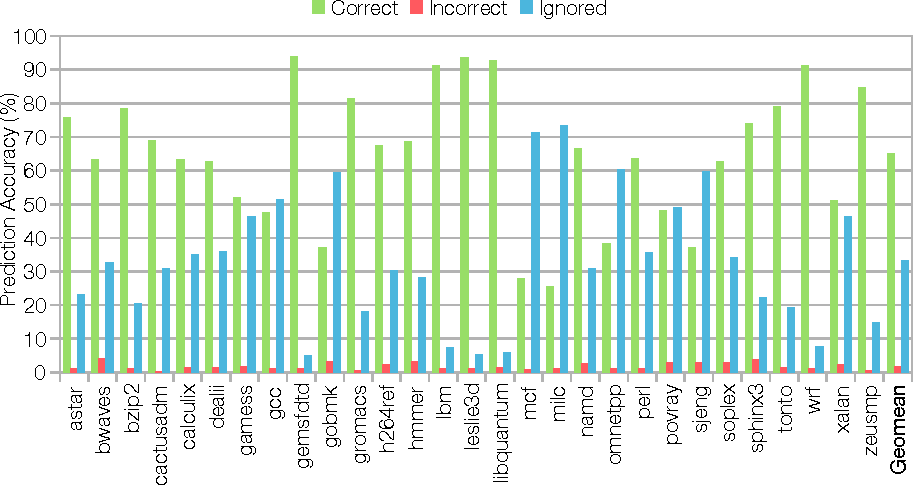
\includegraphics[width=0.50\textwidth]{graphs/ValuePredAccuracy.pdf}}
\caption{Value prediction accuracy for all load addresses}
\label{fig:VPAccuracy}
\end{figure}

While low coverage can only limit the potential of AT-RT technique, incorrect address predictions on the other hand can have a negative impact, since incorrectly forwarded loads will have to be replayed. Figure~\ref{fig:VPAccuracy} also shows ratio of loads that have their address mispredicted. Most benchmarks (20) have a mispredcition ratio bellow 2\% with an average of 1.6\%. 


%\begin{figure}[ht]
%\centerline{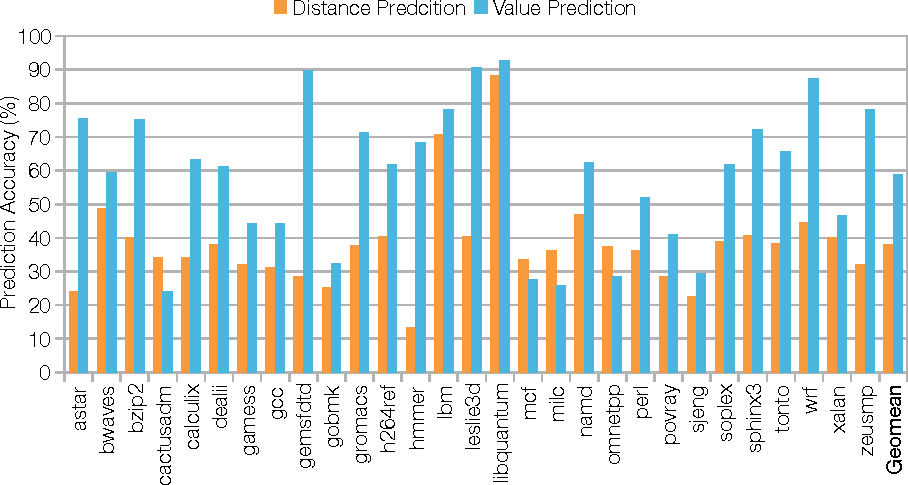
\includegraphics[width=0.50\textwidth]{graphs/DistVsValue.pdf}}
%\caption{Prediction accuracy of using distance and value prediction}
%\label{fig:DistVsValue}
%\end{figure}

%Since the predicted addresses will be used to detect load-to-load forwarding, to contextualised how accurate the prediction is, it also relevant to compare the accuracy with the current state-of-the art heuristic to predict addresses for the same end (ISRB), i.e. \textit{instruction distance} (IDist). Figure~\ref{fig:DistVsValue} compares the accuracy of both strategies at predicting load addresses. The value predictor is more accurate that IDist on 89\% of the benchmarks (25). On the \textit{milc} benchmark is where IDist has the biggest advantage, accurately out-predicting AVP by 10 percentage points. However, overall AVP has a coverage of 59\% compared to the 38\% of IDist, an 1.6x increase.     

%Note the accuracy measured in this graph is not the percentage of loads that have their data forwarded, in the case of IDist technique, the distance might be correct, but it is not possible to forward the data because the older load has left the load-queue.   




\subsection{Load-to-Load Forwarding}
Figure~\ref{fig:Reuse} compares how much load-to-load reuse the different configurations are able to take a advantage off, and how much is exposed by the load queue (i.e. perfect reuse of in-flight loads). The instruction distance configuration (IDist) can forward 16\% of the loads on average with the best benchmark being \textit{lbm} which has 41\% of its loads forwarded from the physical register file. Overall, IDist is able to extract 43\% of the load-to-load locality exposed in the load-queue through the PRF. 

\begin{figure*}[ht]
\centerline{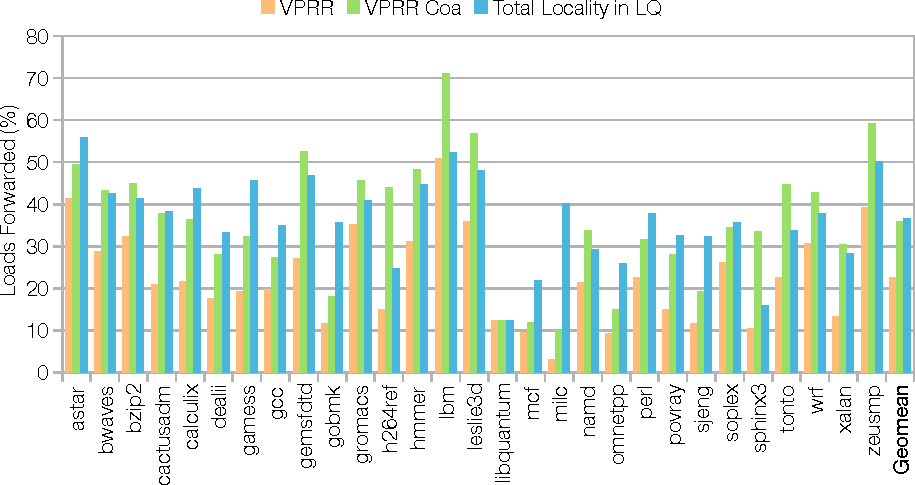
\includegraphics[width=0.99\textwidth]{graphs/RegisterReuse.pdf}}
\caption{Percentage of loads that have their data forwarded from the physical register file}
\label{fig:Reuse}
\end{figure*}

\begin{figure*}[ht]
\centerline{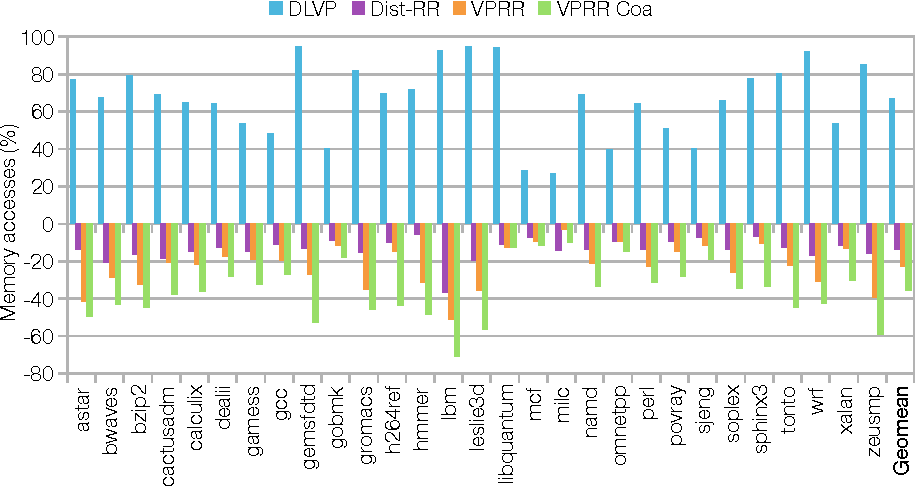
\includegraphics[width=0.99\textwidth]{graphs/MemReduction.pdf}}
\caption{Executed load instructions (L1 accesses by loads) of the different strategies compared to the baseline configuration}
\label{fig:MemReduction}
\end{figure*}

The AT-RT (Temp) configuration is able to forward more data than the IDist on 26 of 29 benchmarks. Of the three benchmarks where AT-RT performs worse than IDist, \textit{milc} shows the highest difference, with the AT-RT forwarding 4 percentage points fewer loads than IDist. The remainder two benchmarks (\textit{dealii} and \textit{leslie3d}), fall behind by less than 1 percentage point (0.7, 0.08 respectively). On the other hand, AT-RT (Temp) shows the biggest gains on \textit{astar}, \textit{cactusadm} and \textit{gromacs} with 25, 18 and 16 percentage point increase over IDist. Overall, AT-RT (Temp) is able to forward 23\% of the loads (1.4x more than IDist) and is able to extract 62\% of the load-to-load locality exposed in the load queue through the PRF.

The AT-RT (Temp+Spac) configuration that fetches data in 128-bit blocks is able to to outperform both the IDist and AT-RT (Temp) across the entire benchmark suite. Benchmarks such as \textit{h264ref}, \textit{sphinx3} and \textit{xalan}, show an improvement of 1.9x, 2.2x and 1.3x compared to AT-RT (temp), and 5x, 5.2x and 3x compared to IDist. 

Since AT-RT (Temp+Spac) takes advantage of the reduced register pressure to extend the lifetime of some registers, it is able to forward more data than what is exposed by the load-queue window. On 14 of the benchmarks, the AT-RT (Temp+Spac) is able surpass the total locality available in load-queue. \textit{Sphinx3} forwards 2.1x more loads than what any load-queue forward predictor can, and \textit{lbm} can forwards 70\% of its loads from the PRF. Overall AT-RT (Temp+Spac) is able to extract 98\% of the load-to-load locality exposed in the load-queue through the PRF.

%\begin{figure}[h]
%\centerline{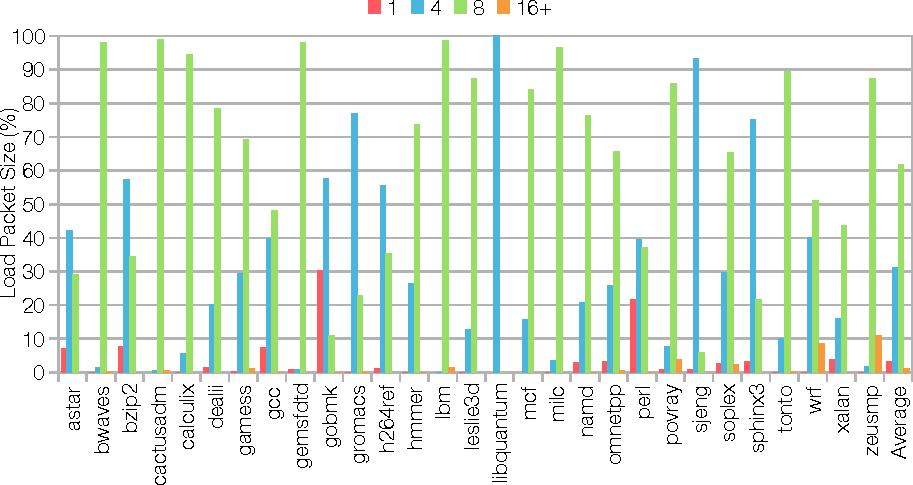
\includegraphics[width=0.50\textwidth]{graphs/PktSize.pdf}}
%\caption{Breakdown of the the data sizes of the loads in the load-queue that can be forwarded.}
%\label{fig:Reuse}
%\end{figure}



\subsection{Memory Access Reduction}
Since DLVP tries to prefetch every address-predicted load instruction, the higher the accuracy of the address predictor, the higher the number of prefetches and thus the the higher the number of loads that need to be replayed. Figure~\ref{fig:MemReduction} shows the increase in L1 accesses by loads from DLVP compared to a standard non-pipeline-prefecthing CPU. On average, DLVP executes 60\% more loads than the baseline and more than 90\% on \textit{gemsfdtd}, \textit{leslie3d} and \textit{libquantum}. The redundant verification load can be filtered by using the SSBF, which would reduce the replays to match the baseline (not shown in the graph) with the exception of the mispredicted prefetches, but those are rare as it can be seen in Figure~\ref{fig:VPAccuracy}.

%\begin{figure*}[h]
%\centerline{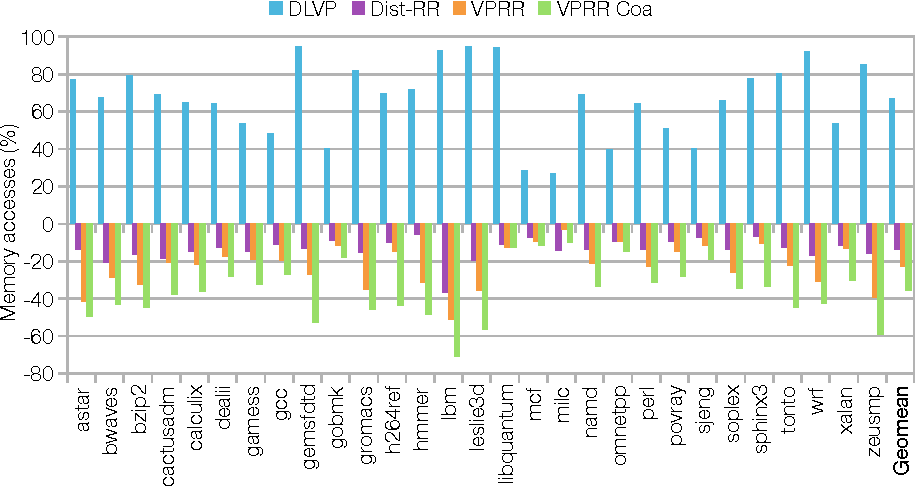
\includegraphics[width=0.99\textwidth]{graphs/MemReduction.pdf}}
%\caption{Executed load instructions (L1 accesses by loads) of the different strategies compared to the baseline configuration}
%\label{fig:MemReduction}
%\end{figure*}

IDist (when extended with SSBF) and both AT-RT strategies can however reduce the number of loads compared to the baseline by not only avoiding the second verification load, but avoid the prefetched one too if it the result is in the PRF. The number of loads that can be filtered is directly related to the ability of the forwarding strategy to detect and take advantge of reuse. AT-RT (Temp) is able to reduce accesses to the memory system by 23\% on average, and up to 51\% in \textit{lbm}. This is an improvement over the 15\% average memory system access reduction of IDist with its highest reduction also being on \textit{lbm} with 41\%. Overall AT-RT (Temp) shows a 1.5x improvement over IDist.

AT-RT (Temp+Spac) shows the biggest improvement and eliminates 36\% of the L1 load accesess compared to the baseline, a 2.4x improvement over IDist. \textit{Lbm} is once again the benchmark with the biggest reduction, by decreasing load execution by 70\%. 











\section{Conclusion}
Recent load value prediction techniques improve IPC by predicting load addresses and prefetching the data into the pipeline. This achieves the same zero load-to-use latency as an all-instruction value predictor but with simpler CPU components making more feasible to implement in hardware. However, it comes with a great increase in pressure in the physical register file and L1 cache in order to validate predictions.

In this work, we make two observations: (1) the value predicted address are special and that the validation of most predicted addresses do not require the load to be replayed to validate the prediction, most of the CPU components required to validate the predicted load are already present in the CPU to detect memory ordering violations; and (2) due to having addresses early in the pipeline, we can easily cache, manage and detect data reuse, and perform load-to-load forwarding through the physical register, further decreasing register and cache pressure.

Our proposed AT-RT address based register reuse technique improves data forwarding through the register file by 2.2x on average compared to a instruction-distance register sharing strategy. Moreover, it not only nullifies the extra load instructions associated with pipeline-prefetching, but it reduces the total number of load instructions executed by 36\%, without compromising any performance benefit associated with DLVP.











%%%%%%%%% -- BIB STYLE AND FILE -- %%%%%%%%
\bibliographystyle{IEEEtranS}
\bibliography{refs}
%%%%%%%%%%%%%%%%%%%%%%%%%%%%%%%%%%%%

\end{document}
